\chapter{\label{sec:perpalyakovetes}Periodikus pályák numerikus követése}

Dinamikai rendszerek vizsgálatánál kíváncsiak vagyunk a rendszer viselkedésére különböző paraméterkombinációk esetében is.
A paraméterek ha\-tá\-sá\-nak vizsgálatára többféle módszer is rendelkezésünkre áll, mint például a paraméterléptetés vagy a pszeudo-ívhossz módszer.
Paraméterléptetés esetén a bifurkációs paraméter értékét kis mértékben megváltoztatjuk, ekkor jól megfogalmazott probléma esetén a megoldás is kis mértékben fog változni, és ezt a változást követjük lépésről-lépésre.
Pszeudo-ívhossz mód\-szer\-nél a bifurkációs paraméter és a periódikus pálya periódusidejének össze\-füg\-gé\-sét keressük oly módon, hogy a problémát egy "szintvonal" keresésre vezetjük vissza.
A fejezetben ez utóbbival fogunk részletesebben foglalkozni.

\section{Pszeudo-ívhossz módszer}
\label{sec:pseudo_ivhossz}

A pszeudo-ívhossz módszer esetében a soron következő megoldást az előző megoldástól $\mathbf{v}$ irányba keressük, ahol $\mathbf{v}$ egy implicit egyenlet $F(\mathbf{x}) = 0$ szintvonalának érintőjével párhuzamos egységhosszú vektor:
\begin{equation}
\begin{cases}
0 = \left< \mathbf{x}_{i+1} - \mathbf{x}_i, \mathbf{v}_i \right> - \Delta s \\
0 = F(\mathbf{x}_{i+1}),
\end{cases}
\label{eq:pszeudo_ivhossz_alapegyenlet}
\end{equation}
\begin{equation}
\mathbf{x_i}= \begin{bmatrix}
x_i & y_i
\end{bmatrix}^\mathrm{T},
\end{equation}
és $\Delta s$ a lépés ívhossza.
Az első egyenlet a merőlegességi feltétel, a második magának a keresett szintvonalnak az egyenlete.
A módszer egy iterációs lépésének szemléltetése a \ref{fig:pszeudo_ivhossz_szemleltet}. ábrán látható.
A merőlegességi feltétel az alábbi módon vezethető le:
\begin{equation}
\hat{\mathbf{x}} = \mathbf{x}_i + \Delta s \, \mathbf{v}_i,
\end{equation}
\begin{equation}
\begin{matrix}
\left< \mathbf{x}_{i+1} - \hat{\mathbf{x}}, \mathbf{v}_i \right> & = & 
\left< \mathbf{x}_{i+1} - \mathbf{x}_i - \Delta s \, \mathbf{v}_i, \mathbf{v}_i \right>  & = \\
\left< \mathbf{x}_{i+1} - \mathbf{x}_i, \mathbf{v}_i \right> - \Delta s \, \left< \mathbf{v}_i , \mathbf{v}_i \right> & = & \left< \mathbf{x}_{i+1} - \mathbf{x}_i, \mathbf{v}_i \right> - \Delta s. & \blacksquare 
\end{matrix}
\end{equation}

\begin{figure}[ht]
	\centering
	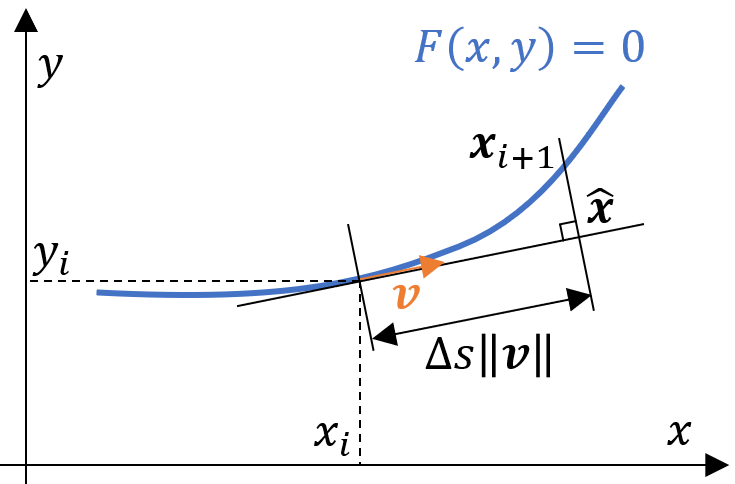
\includegraphics[width=0.4\textwidth]{graphics/pszeudo_ivhossz_szemleltet.png}
	\caption{A pszeudo-ívhossz módszer egy iterációs lépésének szemléltetése}\label{fig:pszeudo_ivhossz_szemleltet}
\end{figure}

A módszer alkalmazása során a \eqref{eq:pszeudo_ivhossz_alapegyenlet} egyenletrendszert szimultán kell megoldani $\mathbf{x}_{i+1}$-re - két egyenlet, két ismeretlen.
A módszer általánosítható több dimenzióra is, ekkor több $F_j(\mathbf{x})$ egyenletre van szük\-sé\-günk.

Egy \textbf{példa} a módszer alkalmazására az egység sugarú kör körívének követése.
Akkor az implicit függvényünk az alábbi:
\begin{equation}
F(\mathbf{x}) = x^2 + y^2 -1.
\end{equation}
A kezdőpontunk legyen
\begin{equation}
\mathbf{x}_0 = \begin{bmatrix}
1 & 0
\end{bmatrix}^\mathrm{T},
\end{equation}
amely, mint látható kielégíti az implicit egyenletünket.
A sebességvektor, azaz az érintő ebben a pontban
\begin{equation}
\mathbf{v}_0 = \begin{bmatrix}
0 & 1
\end{bmatrix}^\mathrm{T}.
\end{equation}
Azonban az esetek többségében ez nem ilyen egyszerűen meghatározható, és numerikusan kell közelítenünk, amihez ismernünk kell a szintvonal egy másik, közeli pontját is, $\mathbf{x}_{1/2}$-et:
\begin{equation}
\mathbf{v}_0 = \frac{\mathbf{x}_{1/2} - \mathbf{x}_{0}}{\left \| \mathbf{x}_{1/2} - \mathbf{x}_{0} \right \|}.
\end{equation}
A sebességvektor ezek után rendre:
\begin{equation}
\mathbf{v}_i = \frac{\mathbf{x}_{i} - \mathbf{x}_{i-1}}{\left \| \mathbf{x}_{i} - \mathbf{x}_{i-1} \right \|}.
\end{equation}
A körív követésének eredménye a pszeudo-ívhossz módszerrel a \ref{fig:pszeudo_ivhossz_koriv}. ábrán látható.
A lépéshossz $\Delta s = 0.1$ volt, a kezdeti sebességbecsléshez az $\mathbf{x}_0$-hoz közeli szintvonal pont pedig
\begin{equation}
\mathbf{x}_{1/2} = \begin{bmatrix}
0.99 & \sqrt{1 - 0.99^2}
\end{bmatrix}^\mathrm{T}.
\end{equation}

\begin{figure}[ht]
	\centering
	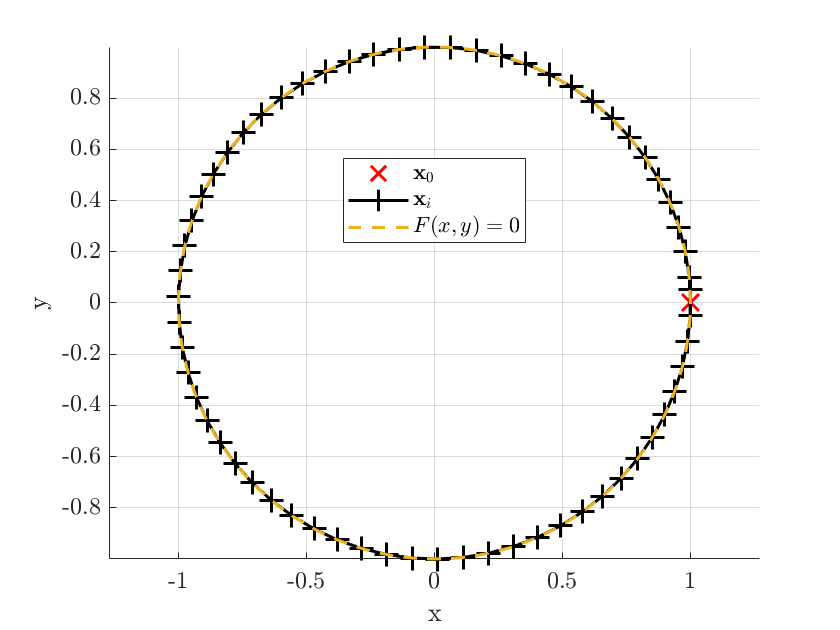
\includegraphics[width=0.8\textwidth]{graphics/pszeudo_ivhossz_koriv}
	\caption{A pszeudo-ívhossz módszer alkalmazása körív követésére}\label{fig:pszeudo_ivhossz_koriv}
\end{figure}

\textbf{Megjegyzés:} pontosabb sebességvektort kapunk az iteráció során, ha a megoldáskor $\mathbf{x}_{i+1/2}$-re is alkalmazzuk a pszeudo-ívhossz módszert, ekkor a sebességvektor általánosan így írható fel:
\begin{equation}
\mathbf{v}_i = \frac{\mathbf{x}_{i+1/2} - \mathbf{x}_{i}}{\left \| \mathbf{x}_{i+1/2} - \mathbf{x}_{i} \right \|}.
\end{equation}
Az így keletkező extra egyenletek ugyanolyan formájúak, mint a \eqref{eq:pszeudo_ivhossz_alapegyenlet} egyenlet az alábbi indexelést alkalmazva a problémára:
\begin{equation}
\begin{cases}
0 = \left< \mathbf{x}_{i+3/2} - \mathbf{x}_{i+1/2}, \mathbf{v}_i \right> - \Delta s \\
0 = F(\mathbf{x}_{i+3/2}),
\end{cases}
\end{equation}
Összességében ez a feladat egy négyváltozós nemlineáris gyökkeresési probléma az eredeti kétváltozós helyett.

\section{Periodikus pályák peremérték-megfogalmazása}
\label{sec:per_palya_perem_megfog}

Dinamikai rendszerek mozgásegyenleteinek megoldásakor kezdeti értéket szoktunk megadni.
Amennyiben a rendszer periódikus mozgást végez, a probléma átírható egy peremérték feladatra, ahol a peremfeltételt a periódus elejére és végére kell előírni.
Belátható ugyanis, hogy periódikus mozgásnál az állapotváltozóknak $t_0$ és $t_0 + T$ időpontokban meg kell egyezniük, ahol $T$ a periódusidő.
Dinamikai rendszerek mozgásegyenleteit Cauchy átírással általánosan az alábbi módon lehet megadni:
\begin{equation}
\dot{\mathbf{z}}(t) = \mathbf{F}(\mathbf{z}(t)),
\label{eq:EOM_altalanosan}
\end{equation}
ahol $\mathbf{z}(t)$ az állapotváltozók, $\mathbf{q}(t)$ pedig az általános koordináták vektora:
\begin{equation}
\mathbf{z}(t) = \begin{bmatrix}
\mathbf{q}(t) & \dot{\mathbf{q}}(t)
\end{bmatrix}^\mathrm{T}.
\end{equation}
Periódikus mozgás esetén (autonóm rendszereknél $t_0$ szabadon megválasztható, így vegyük zérusnak) igaz a következő
\begin{equation}
\mathbf{z}_\mathrm{p}(0) = \mathbf{z}_\mathrm{p}(T) .
\end{equation}

Vezessük be $\tau$ dimenziótlan időt az alábbi módon:
\begin{equation}
\tau =  t/T.
\end{equation}
Ekkor a \eqref{eq:EOM_altalanosan} egyenlet formája és a peremérték feladat a következő lesz
\begin{equation}
\begin{cases}
\mathbf{z}'(\tau) = T\,\mathbf{F}(\mathbf{z}(\tau)), \\
\mathbf{z}(0) = \mathbf{z}(1).
\end{cases}
\label{eq:EOM_dimtalan}
\end{equation}

\textbf{Megjegyzés:} amennyiben a rendszerünk szakaszosan folytonos a \eqref{eq:EOM_dimtalan}-es problémát ki kell egészíteni:
\begin{equation}
\begin{matrix}
\begin{cases}
\mathbf{z}'(\tau_1) = T_1\,\mathbf{F}_1(\mathbf{z}(\tau_1)), \; H(\mathbf{z}(\tau_1)) > 0,\\
\mathbf{z}'(\tau_2) = T_2\,\mathbf{F}_2(\mathbf{z}(\tau_2)), \; H(\mathbf{z}(\tau_2)) < 0,
\end{cases} \\\\
\begin{cases}
\mathbf{z}_1(1) = \mathbf{z}_2(0), \\
\mathbf{z}_2(1) = \mathbf{z}_1(0),
\end{cases} \\\\
\begin{cases}
H(\mathbf{z}_1(1)) = 0, \\
H(\mathbf{z}_2(1)) = 0,
\end{cases}
\end{matrix}
%\label{eq:EOM_dimtalan}
\end{equation}
ahol $H(\mathbf{z}(\tau))$  a kapcsolófelület.
Ütköző rendszer esetében figyelembe kell venni a peremfeltételek felírásánál az ütközéskor létrejövő leképezést.

Nézzük meg egy egyszerű \textbf{példa} peremérték-megfogalmazásának implementálását MATLAB környezetben!
Peremérték feladatok megoldására a bvp beépített megoldókat lehet használni, esetünkben a bvp5c-vel fogunk dolgozni.
A mechanikai rendszerünk a \ref{fig:bvp_tomeg_rugo}. ábrán látható.

\begin{figure}[ht]
	\centering
	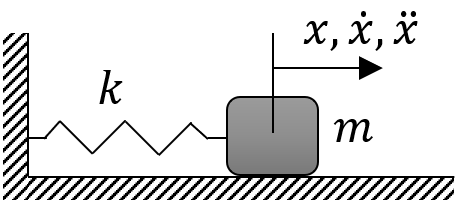
\includegraphics[width=0.3\textwidth]{graphics/tomeg_rugo_modell}
	\caption{Periódikus mozgást végző tömeg-rugó rendszer}\label{fig:bvp_tomeg_rugo}
\end{figure}

A mozgásegyenlete a fenti rendszernek jól ismert:
\begin{equation}
\ddot{x}= -\frac{k}{m}\,x.
\end{equation}
Mint tudjuk, a rendszer mozgását leíró függvényt az alábbi módon lehet felírni, amennyiben $x_0$ kezdeti kitérítésünk van csak $\tau_0$ időpillanatban kezdeti sebesség nélkül:
\begin{equation}
\varphi(\tau) = x_0\cos\left(\tau\sqrt{k/m}\,T\right) = x_0\cos\left(2\pi\,\tau\right),
\end{equation}
\begin{equation}
\dot{\varphi}(\tau) = -x_0\sqrt{k/m}\sin\left(\tau\sqrt{k/m}\,T\right) = -x_0\sqrt{k/m}\sin\left(2\pi\,\tau\right),
\end{equation}
ahol $T$ a rendszer sajátfrekvenciájának inverze
\begin{equation}
T = 2\pi\sqrt{m/k}.
\end{equation}
A fenti függvényeket a peremérték-megfogalmazáskor kijöttekkel fogjuk összevetni.

A bvp5c megoldóhoz először definiálnunk kell egy időrácsot, amely i\-dő\-pon\-tok\-ban meg kell becsülnünk majd a keresett függvények értékét.
Mivel áttértünk dimenziótlan időre, egy periódus "peremei" a $\tau \in \left \{ 0,1 \right \}$ pontok, valamint megjelent a Cauchy átírásnál $T$ periódusidő, mint ismeretlen paraméter.
\begin{equation}
\begin{bmatrix}
x'(\tau) \\ y'(\tau)
\end{bmatrix} = 
T
\begin{bmatrix}
y(\tau) \\  -\frac{k}{m}\,x(\tau)
\end{bmatrix} 
\end{equation}
A módszer a rácsháló első és utolsó pontjára fogja alkalmazni a peremfeltételeket.
Jó kezdeti függvénybecslés a megoldó megfelelő működéséhez az egyik legfontosabb kritérium, ehhez minél több információt össze kell gyűjteni a vizsgált rendszer viselkedéséről.
A kezdeti függvénybecslésnek teljesítenie kell a peremfeltételeket.%, melyeknek rajta kell lenniük a periódikus pályán.
Az ismeretlen paraméter(ek)re is szükséges kezdeti becslést adni!
A peremfeltételeket megadó vektor (res $\in \mathbb{R}^r = \mathbb{R}^{n+p}$) dimenziója megegyezik a mozgásegyenlet (dydx $\in \mathbb{R}^n$) és a paramétereket tartalmazó vektor (par $\in \mathbb{R}^p$) dimenziójának összegével.
\begin{lstlisting}
global k m x0
k = 10;
m = 5;
x0 = 1;
taumesh = linspace(0,1,5);
par = 2*pi;
solinit = bvpinit(taumesh, @bvp_initial_guess, par);
sol = bvp5c(@bvp_fun, @bvp_bcs, solinit);

function g = bvp_initial_guess(x)
global x0
g = x0*[cos(2*pi*x); -2*pi*sin(2*pi*x)];
end

function dydx = bvp_fun(x,y,par)
global k m
dydx = par*[y(2); -k*y(1)/m];
end

function res = bvp_bcs(ya,yb,par)
global x0
res = [ya(1) - x0
    yb(1) - x0
    ya(2)];
end
\end{lstlisting}

A módszer által kiszámolt $T$ értéke megegyezik az analitikusan kiszámított periódusidővel.
A tömegpont pozíciója és sebessége a \ref{fig:bvp_tomeg_rugo_traj_vel}. ábrán látható.

\begin{figure}[ht]
	\centering
	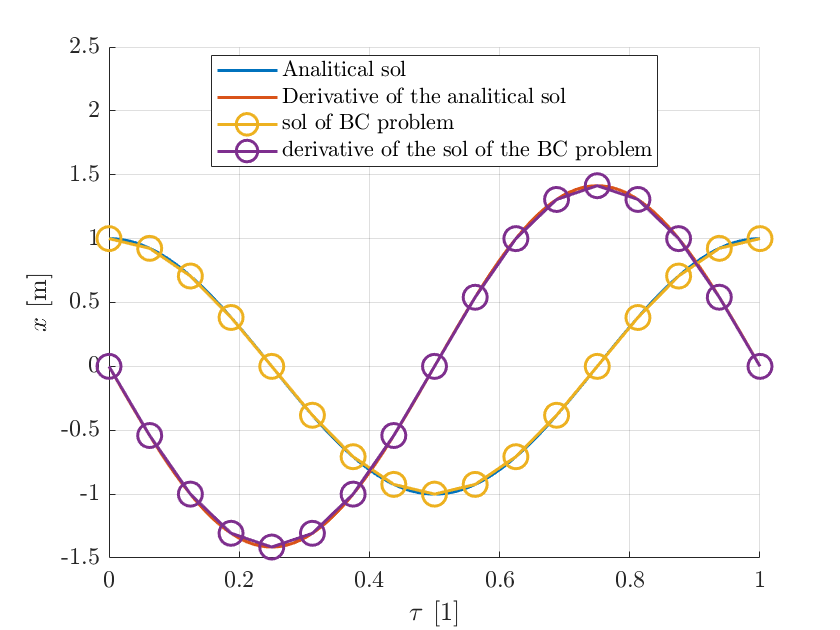
\includegraphics[width=0.75\textwidth]{graphics/BVP_tomeg_rugo}
	\caption{Tömeg-rugó rendszer peremérték-megfogalmazásának bvp5c megoldóval kiszámított eredményeinek összevetése az analitikus megoldással}\label{fig:bvp_tomeg_rugo_traj_vel}
\end{figure}

\section{Pszeudo-ívhossz módszer alkalmazása periodikus pályák kö\-ve\-té\-sé\-hez}

Ebben az alfejezetben két példát nézünk meg, ahol a pszeudo-ívhossz mód\-szert periódikus pályák követésére használjuk.
Ehhez ki kell választanunk majd egy bifurkációs paramétert, amely függvényében kíváncsiak vagyunk, hogyan alakul a periódikus mozgás.
Az első feladat során az előbb vizsgált tömeg-rugó rendszerrel foglalkozunk, a másodikban egy szakaszosan folytonos rendszert, a spring loaded inverted pendulom (SLIP) modellt vizsgáljuk, amely az emberi futás leírásának egy elterjedten használt modellje.

\subsection{Példa 1: tömeg-rugó rendszer}

A pszeudo-ívhossz módszer használatához ki kell választanunk egy bi\-fur\-ká\-ci\-ós paramétert, amit jelöljön $\mu$.
A példa során először vizsgáljuk a rugómerevség $(\mu = k)$, később a tömeg $(\mu =m)$ hatását (ilyenkor a többi paraméter konstans).
A \eqref{eq:pszeudo_ivhossz_alapegyenlet} egyenlet alakja paraméterkövetés során az alábbi formájú:
\begin{equation}
\begin{cases}
0 = \left< \mathbf{x}_{i+1} - \mathbf{x}_i, \mathbf{v}_i \right> - \Delta s \\
0 = T_{i+1} - T_{\mathrm{BVP}}(\mu_{i+1}),
\end{cases}
\label{eq:pszeudo_per_kov}
\end{equation}
\begin{equation}
\mathbf{x_i}= \begin{bmatrix}
\mu_{i} & T_{i}
\end{bmatrix}^\mathrm{T},
\end{equation}
ahol $T_{\mathrm{BVP}}(\mu_{i+1})$ a peremfeladat megoldó által számolt periódusidő.
A psze\-u\-do-ív\-hossz módszert a \ref{sec:pseudo_ivhossz} alfejezetben bemutatott módon kell alkalmazni, és a benne található $T_{\mathrm{BVP}}(\mu_{i+1})$ értékét a \ref{sec:per_palya_perem_megfog} alfejezetben leírt módon kell meghatározni a \eqref{eq:pszeudo_per_kov} egyenletrendszer megoldása közben.
A kapott eredményeket összevetettük az analitikusan kiszámítottakkal, és látható, hogy a pályakövetés illeszkedik az analitikusan előállított görbékre, ld. \ref{fig:pszeudo_tomeg_rugo_k}. és \ref{fig:pszeudo_tomeg_rugo_m}. ábrák.

\begin{figure}[ht]
	\centering
	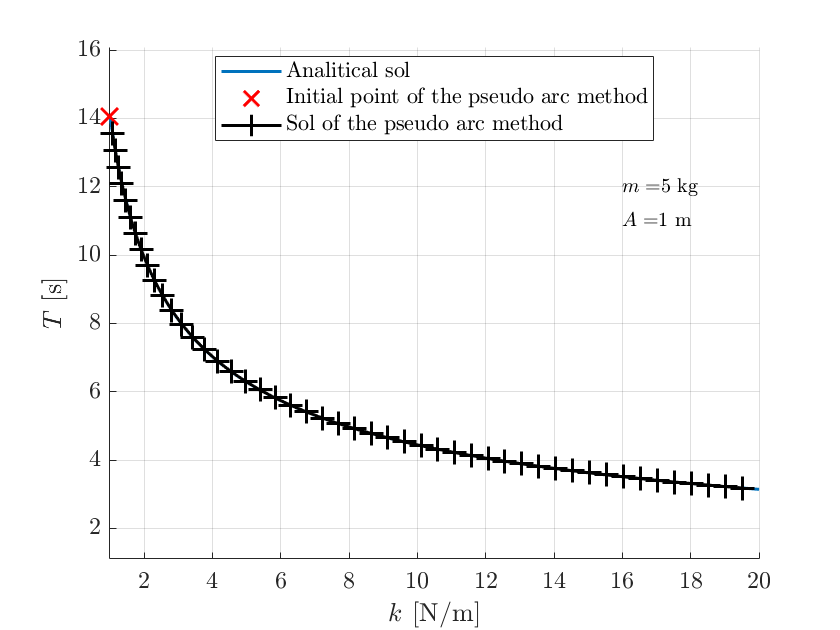
\includegraphics[width=0.9\textwidth]{graphics/pszeudo_tomeg_rugo_k}
	\caption{Periódikus pályák követése $k$ paraméter függvényében, $\Delta s = 0.5$}\label{fig:pszeudo_tomeg_rugo_k}
\end{figure}

\begin{figure}[ht]
	\centering
	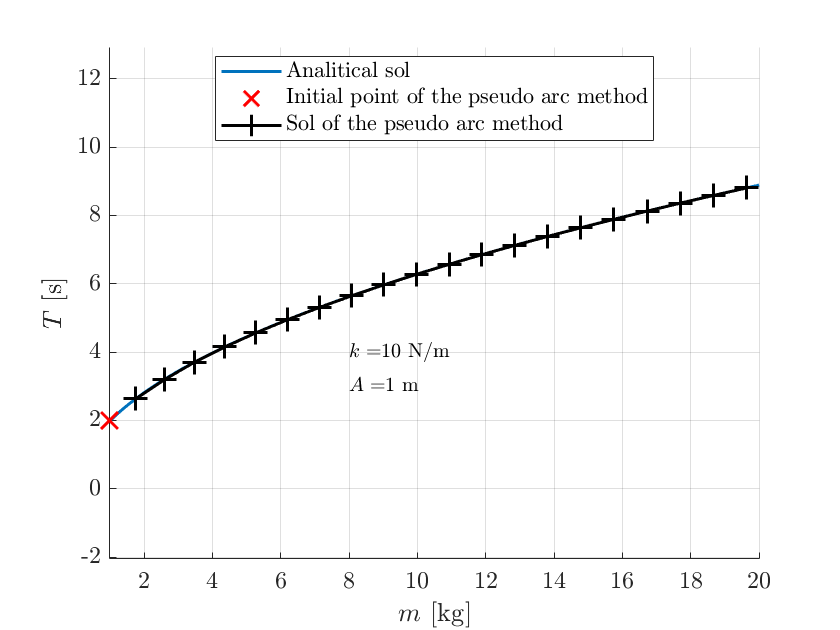
\includegraphics[width=0.9\textwidth]{graphics/pszeudo_tomeg_rugo_m}
	\caption{Periódikus pályák követése $m$ paraméter függvényében, $\Delta s = 1$}\label{fig:pszeudo_tomeg_rugo_m}
\end{figure}

\subsection{Példa 2: spring loaded inverted pendulom modell}

A spring loaded inverted pendulum (SLIP) modell a \ref{fig:SLIP_mechanikai_modell}. ábrán látható.
A rendszer egy tömegpontból és egy tömeg nélküli rugóból áll, ami $\alpha$ szögben kapcsolódik a tömegponthoz.
A SLIP modell az emberi futás modellezéséhez használt egyszerű mechanikai modell.
Periódikus mozgásra képes, mely mozgás két fázisra, a támasz és repülő fázisokra tagolódik, így a rendszer szakaszosan, de $\mathrm{C}^2$ folytonos.

\begin{figure}[ht]
	\centering
	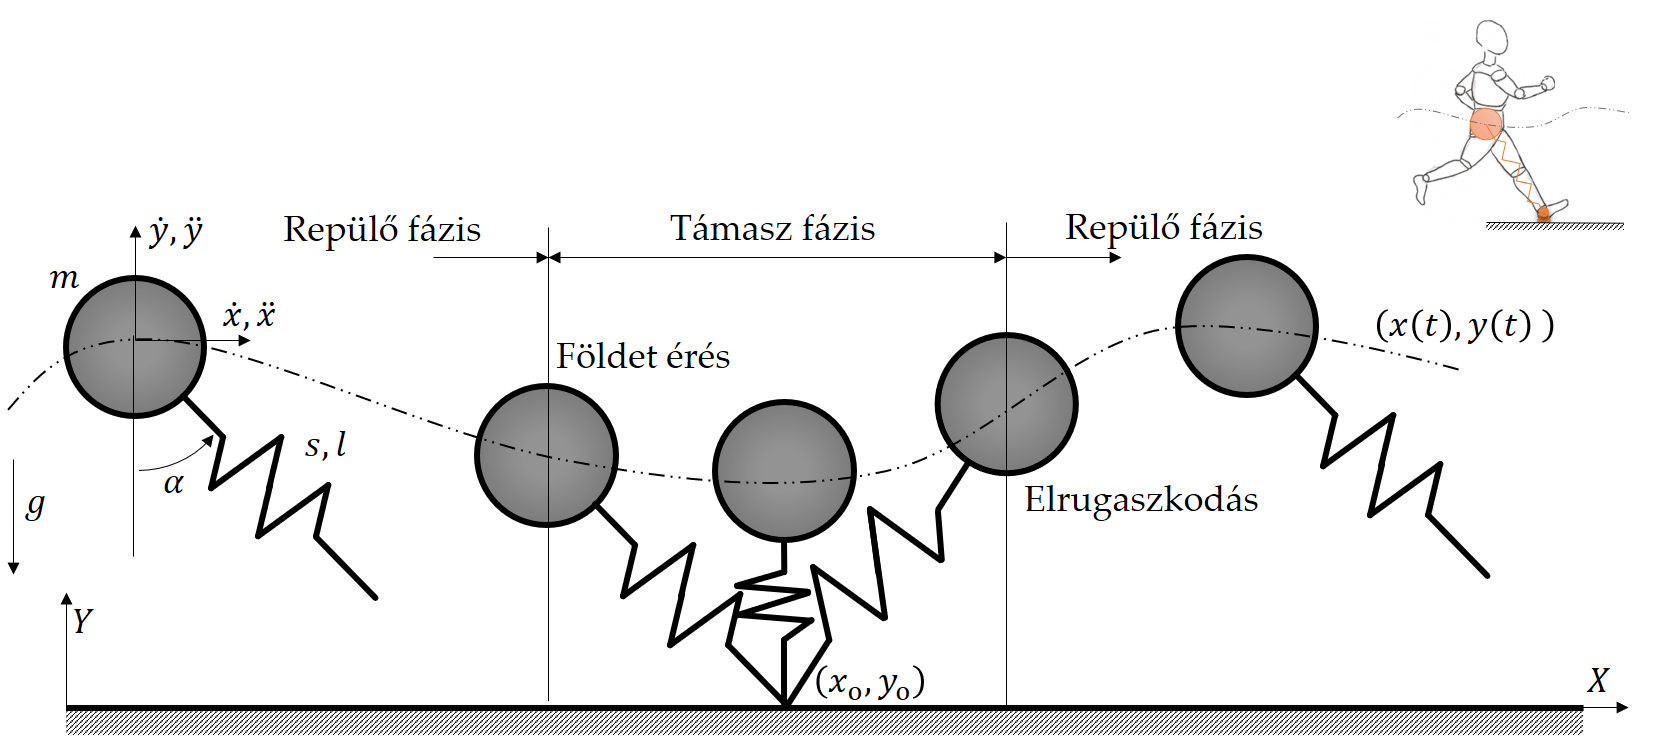
\includegraphics[width=0.9\textwidth]{graphics/slip_mozgas}
	\caption{Spring loaded inverted pendulum (SLIP) mechanikai modellje}\label{fig:SLIP_mechanikai_modell}
\end{figure}

A rendszer mozgásegyenlete a támaszfázisban (mivel az $x$ kvázi ciklikus koordináta (a kezdeti értéke nem befolyásolja a mozgás minőségét, amennyiben a repülőfázisból vagy fá\-zis\-ha\-tá\-rok\-ról indítjuk a rendszert), a rugó megfogott végét önkényesen mindig az origóba helyezzük, ami a tömegpont $x$ koordináta szerinti helyzetét is megadja a fázis elején), és az állapotváltozók az alábbiak:
\begin{equation}
\begin{cases}
\ddot{x} = \kappa\left(l_0 - l(t) \right)x(t)/l(t),\\
\ddot{y} = \kappa\left(l_0 - l(t) \right)y(t)/l(t) - g,
\end{cases}
\end{equation}
\begin{equation}
\mathbf{z}(t)= \begin{bmatrix}
x(t) & y(t) & \dot{x}(t) & \dot{y}(t)
\end{bmatrix}^\mathrm{T},
\end{equation}
\begin{equation}
l(t) = \sqrt{\left(-x(t)\right)^2 + y(t)^2},
\end{equation}
A repülő fázisban is a fenti mozgásegyenlet érvényes, csupán a $\kappa = s/m = 0$ helyettesítést kell alkalmazni.
A fázishatárokat megadó eseményfüggvények a támasz-repülő fázishatáron, illetve a repülő-támasz fázishatáron az a\-láb\-bi\-ak, ahol az 1-es index a támaszfázis, a 2-es a repülőre vonatkozik:
\begin{equation}
\begin{matrix}
H_{12}(\mathbf{z}) = l_0 - l(t), \\
H_{21}(\mathbf{z}) = y(t) - l_0\cos(\alpha).
\end{matrix}
\end{equation}

A peremfeladat megoldásához a mozgásegyenletekre alkalmazni kell a Cauchy-átírást, illetve dimenziótlanítani kell idő szerint.
Külön kell dimenziótlanítani a támaszfázis mozgásegyenleteit a $\tau_1 = t/T_1$ dimenziótlan idővel felírva, és külön a repülőfázisét $\tau_2 = t/T_2$-vel.
\begin{equation}
\begin{matrix}
\begin{cases}
\mathbf{z}'(\tau_1) = T_1\,\mathbf{F}_1(\mathbf{z}(\tau_1)), \; H_{12}(\mathbf{z}(\tau_1)) > 0, \\
\mathbf{z}'(\tau_2) = T_2\,\mathbf{F}_2(\mathbf{z}(\tau_2)), \; H_{21}(\mathbf{z}(\tau_2)) > 0,
\end{cases} \\\\
\begin{cases}
\mathbf{z}_1(1) = \mathbf{z}_2(0), \\
\hat{\mathbf{z}}_2(1) = \hat{\mathbf{z}}_1(0),
\end{cases} \\\\
H_{12}(\mathbf{z}_1(1)) = 0,
 \\\\
x_1(0) = -l_0\sin{\alpha},
\\\\
\hat{E} = l_0\cos(\alpha)\,g + \left(x'_2(1)^2 + y'_2(1)^2\right)/2,
\end{matrix}
\end{equation}
ahol
\begin{equation}
	\hat{\mathbf{z}}(\tau) = 
	\begin{bmatrix}
		y(\tau) & x'(\tau) & y'(\tau)
	\end{bmatrix}^\mathrm{T},
\end{equation}
ugyanis $x(\tau)$ kvázi ciklikus koordináta, melynek értéke periódikus mozgás során szigorú monoton nő, így $\mathbf{z}_1(0)\neq\mathbf{z}_2(1)$, viszont $x_1(0)$ ismert.
Valamint $\hat{E}$ a tömeg szerint fajlagosított mechanikai összenergia, amely a rendszer egy paramétere, hiszen a modell konzervatív.
A $H_{21}(\mathbf{z}_2(1))$ helyett azért jobb a fenti egyenlet használata, mivel ez a kapcsolófelület által tartalmazott információn felül többet mondd, és kijelöli, hogy milyen energiaszinten mozog a rendszer.
A \eqref{eq:pszeudo_per_kov} egyenletben a $T_{\mathrm{BVP}}(\mu_{i+1}) = T_{\mathrm{BVP,1}}(\mu_{i+1}) + T_{\mathrm{BVP,2}}(\mu_{i+1})$ helyettesítést kell alkalmazni a peremfeladat megoldása után.

Egy jó próbafüggvény megadásához először inicializáljuk a feladatot, azaz keresünk egy periódikus pályát.
A feladatot a támaszfázis elejéről indítjuk, és itt $y_1(0) = l_0\cos(\alpha)$ ismert, valamint $x(\tau)$ kvázi ciklikus koordináta.
Mivel a rendszer konzervatív a mechanikai összenergiát paraméternek választva a sebességkomponensek kifejezhetők egymásból a támaszfázis elején, mi a $\dot{x}_1(0)$-t vesszük most független változónak.
A rendszer mozgását tehát adott paraméterkombinációnál egy változó fogja befolyásolni a támaszfázis bal oldali peremén.
Az inicializálásnál az alábbi egyenlet zérushelyét keressük meg:
\begin{equation}
	f(\dot{x}_1(0)) = \dot{x}_1(0) - \dot{x}_2(1) = 0.
\end{equation}
Az inicializált kezdeti próbafüggvényekben a periódikus pálya pontjait hasz\-nál\-juk fel, ahol az időpillanatokat az $xini$, a függvényértékeket az $yini$ változókba mentjük.
Az inicializált kezdeti próbafüggvények a $\dot{x}_1(0) = 5.1149\; \mathrm{m/s}$ kezdeti értékű pe\-ri\-ó\-di\-kus pályához vannak felírva, ahol a paraméterek értéke $l_0 = 1 \; \mathrm{m}$, $\kappa = 112.5\;\mathrm{N/(m\,kg)}$, $\alpha = 0.5708 \;\mathrm{rad}$, $\hat{E} = 21.5 \;\mathrm{N/kg}$.
A pszeudo-ívhossz iterációjában az $xini$ és $yini$ változókat mindig aktualizáljuk a peremfeladat megoldó által számított megoldással.
Fel\-té\-te\-lez\-zük, hogy a változás a pálya képében folyamatos a paraméterek változásával. 
A MATLAB kód lényeges részei lentebb megtekinthetők.
\begin{lstlisting}
for i = 1:imax	
xi_p = start_pseudo_root_finding();	
v = (xi_p-xi)/norm((xi_p-xi));	
xi = xi_p;
end
\end{lstlisting}
\begin{lstlisting}
function y = start_pseudo_root_finding()
mu = xi(1);	
fun_PAM = @pseudo_root_finding;
x = fzero(fun_PAM,mu);	
T_par1 = T_BVP(1);
T_par2 = T_BVP(2);
[T_BVP_1,T_BVP_2]=boundary_SLIP(T_par1,T_par2);
T_BVP=[T_BVP_1,T_BVP_2,T_BVP_1+T_BVP_2];	
y = [x; T_BVP(3)];
end
\end{lstlisting}

\begin{lstlisting}
function y = pseudo_root_finding(mu)
T_par1 = T_BVP(1);
T_par2 = T_BVP(2);
[T_BVP_1, T_BVP_2]  = boundary_SLIP(T_par1, T_par2);
T_BVP = [T_BVP_1, T_BVP_2, T_BVP_1 + T_BVP_2];	
a = v(1);
b = v(2);
c = xi(1);
d = xi(2);	
T_i = (h - (mu - c)*a)/b + d;	
y = T_i - T_BVP(3);
end
\end{lstlisting}
\begin{lstlisting}
function [T1, T2] = boundary_SLIP(T_in1, T_in2)
global xdot10
global xini yini	
xinit = xini;
par = [T_in1; T_in2];
solinit = bvpinit(xinit, @bvp_initial_guess, par);
sol = bvp5c(@bvp_fun, @bvp_bcs, solinit);
T1 = sol.parameters(1);
T2 = sol.parameters(2);
xini = sol.x;
yini = sol.y;
xdot10 = sol.y(3,1);
end

function G = bvp_initial_guess(t)
global xini yini
G = [interp1(xini,yini(1,:),t)
interp1(xini,yini(2,:),t,`spline`)
interp1(xini,yini(3,:),t,`spline`)
interp1(xini,yini(4,:),t,`spline`)
interp1(xini,yini(5,:),t)
interp1(xini,yini(6,:),t,`spline`)
interp1(xini,yini(7,:),t)
interp1(xini,yini(8,:),t)];
end

function dydx = bvp_fun(t,Y,par)
global kappa_f g l0
lambda = sqrt((-Y(1))^2 + (Y(2))^2)/l0;
dydx = [par(1)*Y(3) 
par(1)*Y(4)
par(1)*( (kappa_f/lambda - kappa_f)*Y(1) )
par(1)*( (kappa_f/lambda - kappa_f)*Y(2) - g )
par(2)*Y(7)
par(2)*Y(8)
par(2)*0
-par(2)*g];
end

function res = bvp_bcs(ya,yb,par)
global l0 alpha_f 
global E_f g
res = [ya(1) + l0*sin(alpha_f)
ya(2) - yb(6)
ya(3) - yb(7)
ya(4) - yb(8)
ya(5) - yb(1)
ya(6) - yb(2)
ya(7) - yb(3)
ya(8) - yb(4)
l0 - sqrt((yb(1))^2 + (yb(2))^2) 
E_f - l0*cos(alpha_f)*g - (ya(3)^2 + ya(4)^2)/2];
end

\end{lstlisting}

A rendszer paraméterei a $\kappa$, $\alpha$, $l_0$ és $\hat{E}$, melyek közül tekintsük az $l_0$-t fixen egységnyinek.
A másik három paramétert egyenként fogjuk bifurkációs paraméterként kezelni.
A pszeudo-ívhossz módszer által megvalósított pályakövetés eredményei a \ref{fig:pszeudo_SLIP_E}., \ref{fig:pszeudo_SLIP_kappa}. és \ref{fig:pszeudo_SLIP_alpha}. ábrákon láthatók.

\begin{figure}[ht]
	\centering
	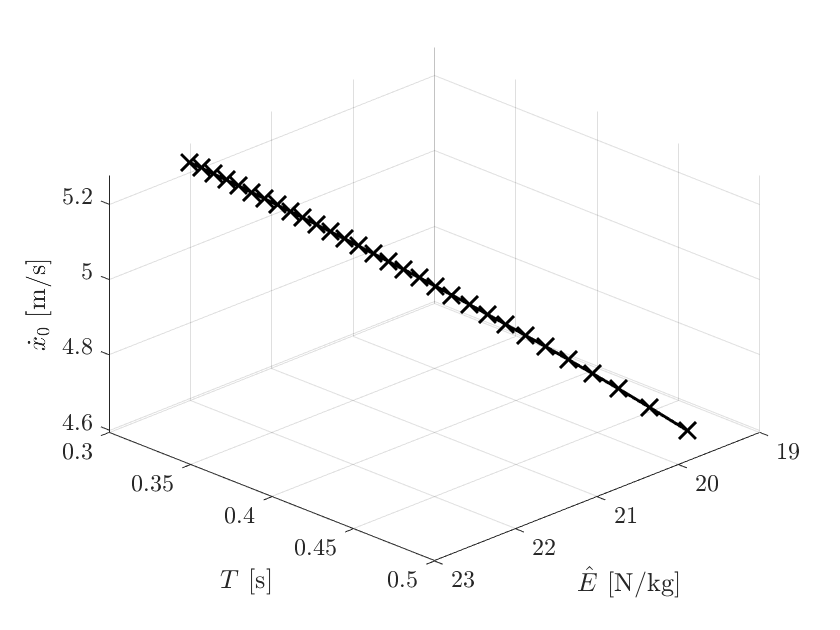
\includegraphics[width=0.8\textwidth]{graphics/pszeudo_SLIP_E}
	\caption{Pszeudó-ívhossz módszer pályakövetése, $\mu = \hat{E}$}\label{fig:pszeudo_SLIP_E}
\end{figure}

\begin{figure}[ht]
	\centering
	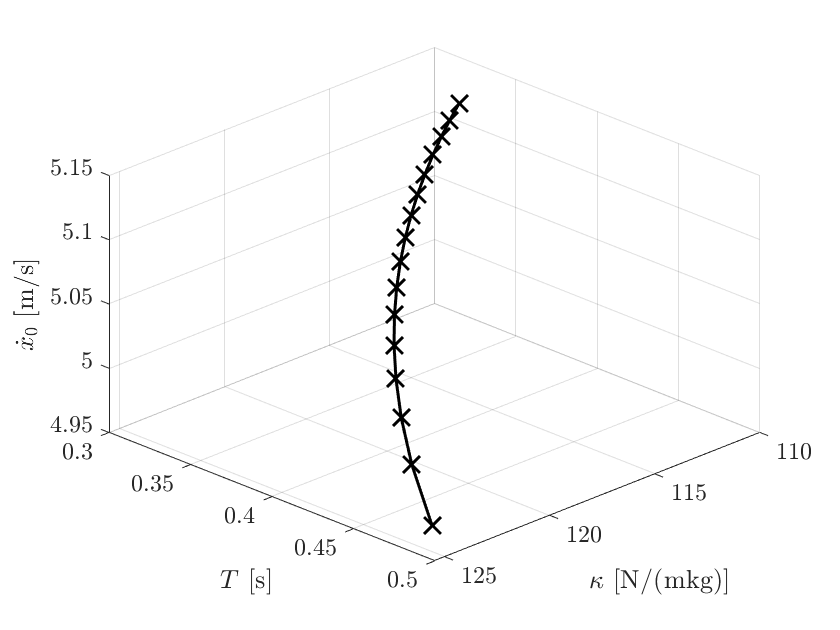
\includegraphics[width=0.8\textwidth]{graphics/pszeudo_SLIP_kappa}
	\caption{Pszeudó-ívhossz módszer pályakövetése, $\mu = \kappa$}\label{fig:pszeudo_SLIP_kappa}
\end{figure}

\begin{figure}[ht]
	\centering
	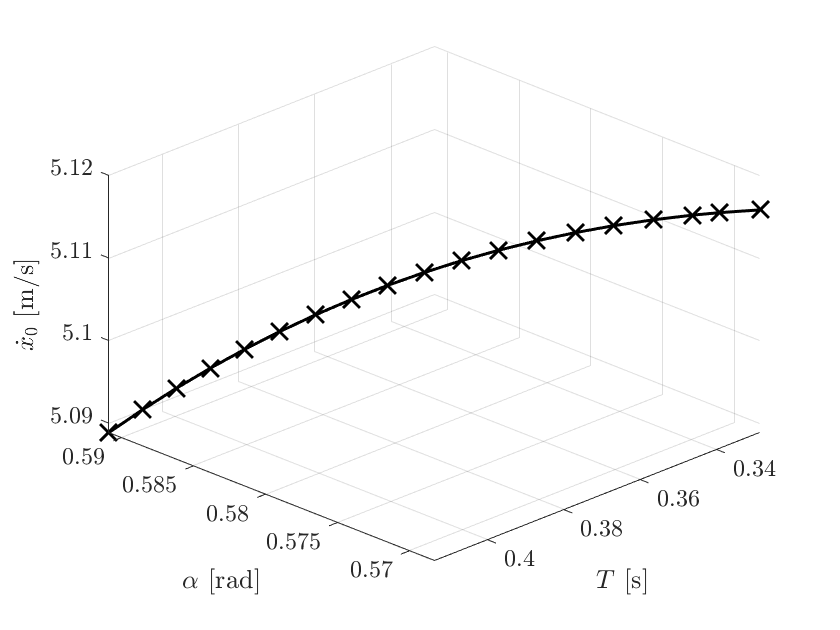
\includegraphics[width=0.8\textwidth]{graphics/pszeudo_SLIP_alpha}
	\caption{Pszeudó-ívhossz módszer pályakövetése, $\mu = \alpha$}\label{fig:pszeudo_SLIP_alpha}
\end{figure}

\textbf{Megjegyzés:} A \eqref{eq:pszeudo_per_kov} egyenletrendszer kipótolható egy harmadik egyenlettel, ami vonatkozhat a monodrómia mátrix sajátértékére; például kereshetjük azt a görbét, ami a stabilitáshatárt mondja meg, azaz amikor a nem triviális sajátérték $\lambda = 1$. Ekkor a mechanikai összeenergia már nem tekinthető paraméternek.
\begin{equation}
\begin{cases}
0 = \left< \mathbf{x}_{i+1} - \mathbf{x}_i, \mathbf{v}_i \right> - \Delta s, \\
0 = T_{i+1} - T_{\mathrm{BVP}}(\mu_{i+1}), \\
0 = 1 - \lambda,
\end{cases}
\end{equation}
\begin{equation}
\mathbf{x_i}= \begin{bmatrix}
\mu_{i} & T_{i} & \lambda_i
\end{bmatrix}^\mathrm{T},
\end{equation}
